\documentclass[12pt]{article}

\usepackage[]{inputenc}
\usepackage{graphicx}

\begin{document}

\title{Supplementary material for "XXX Title"}
\author{Eric Bazin, Keurcien Luu, Michael G. B. Blum}

\maketitle

\begin{figure*}[t]
\begin{center}
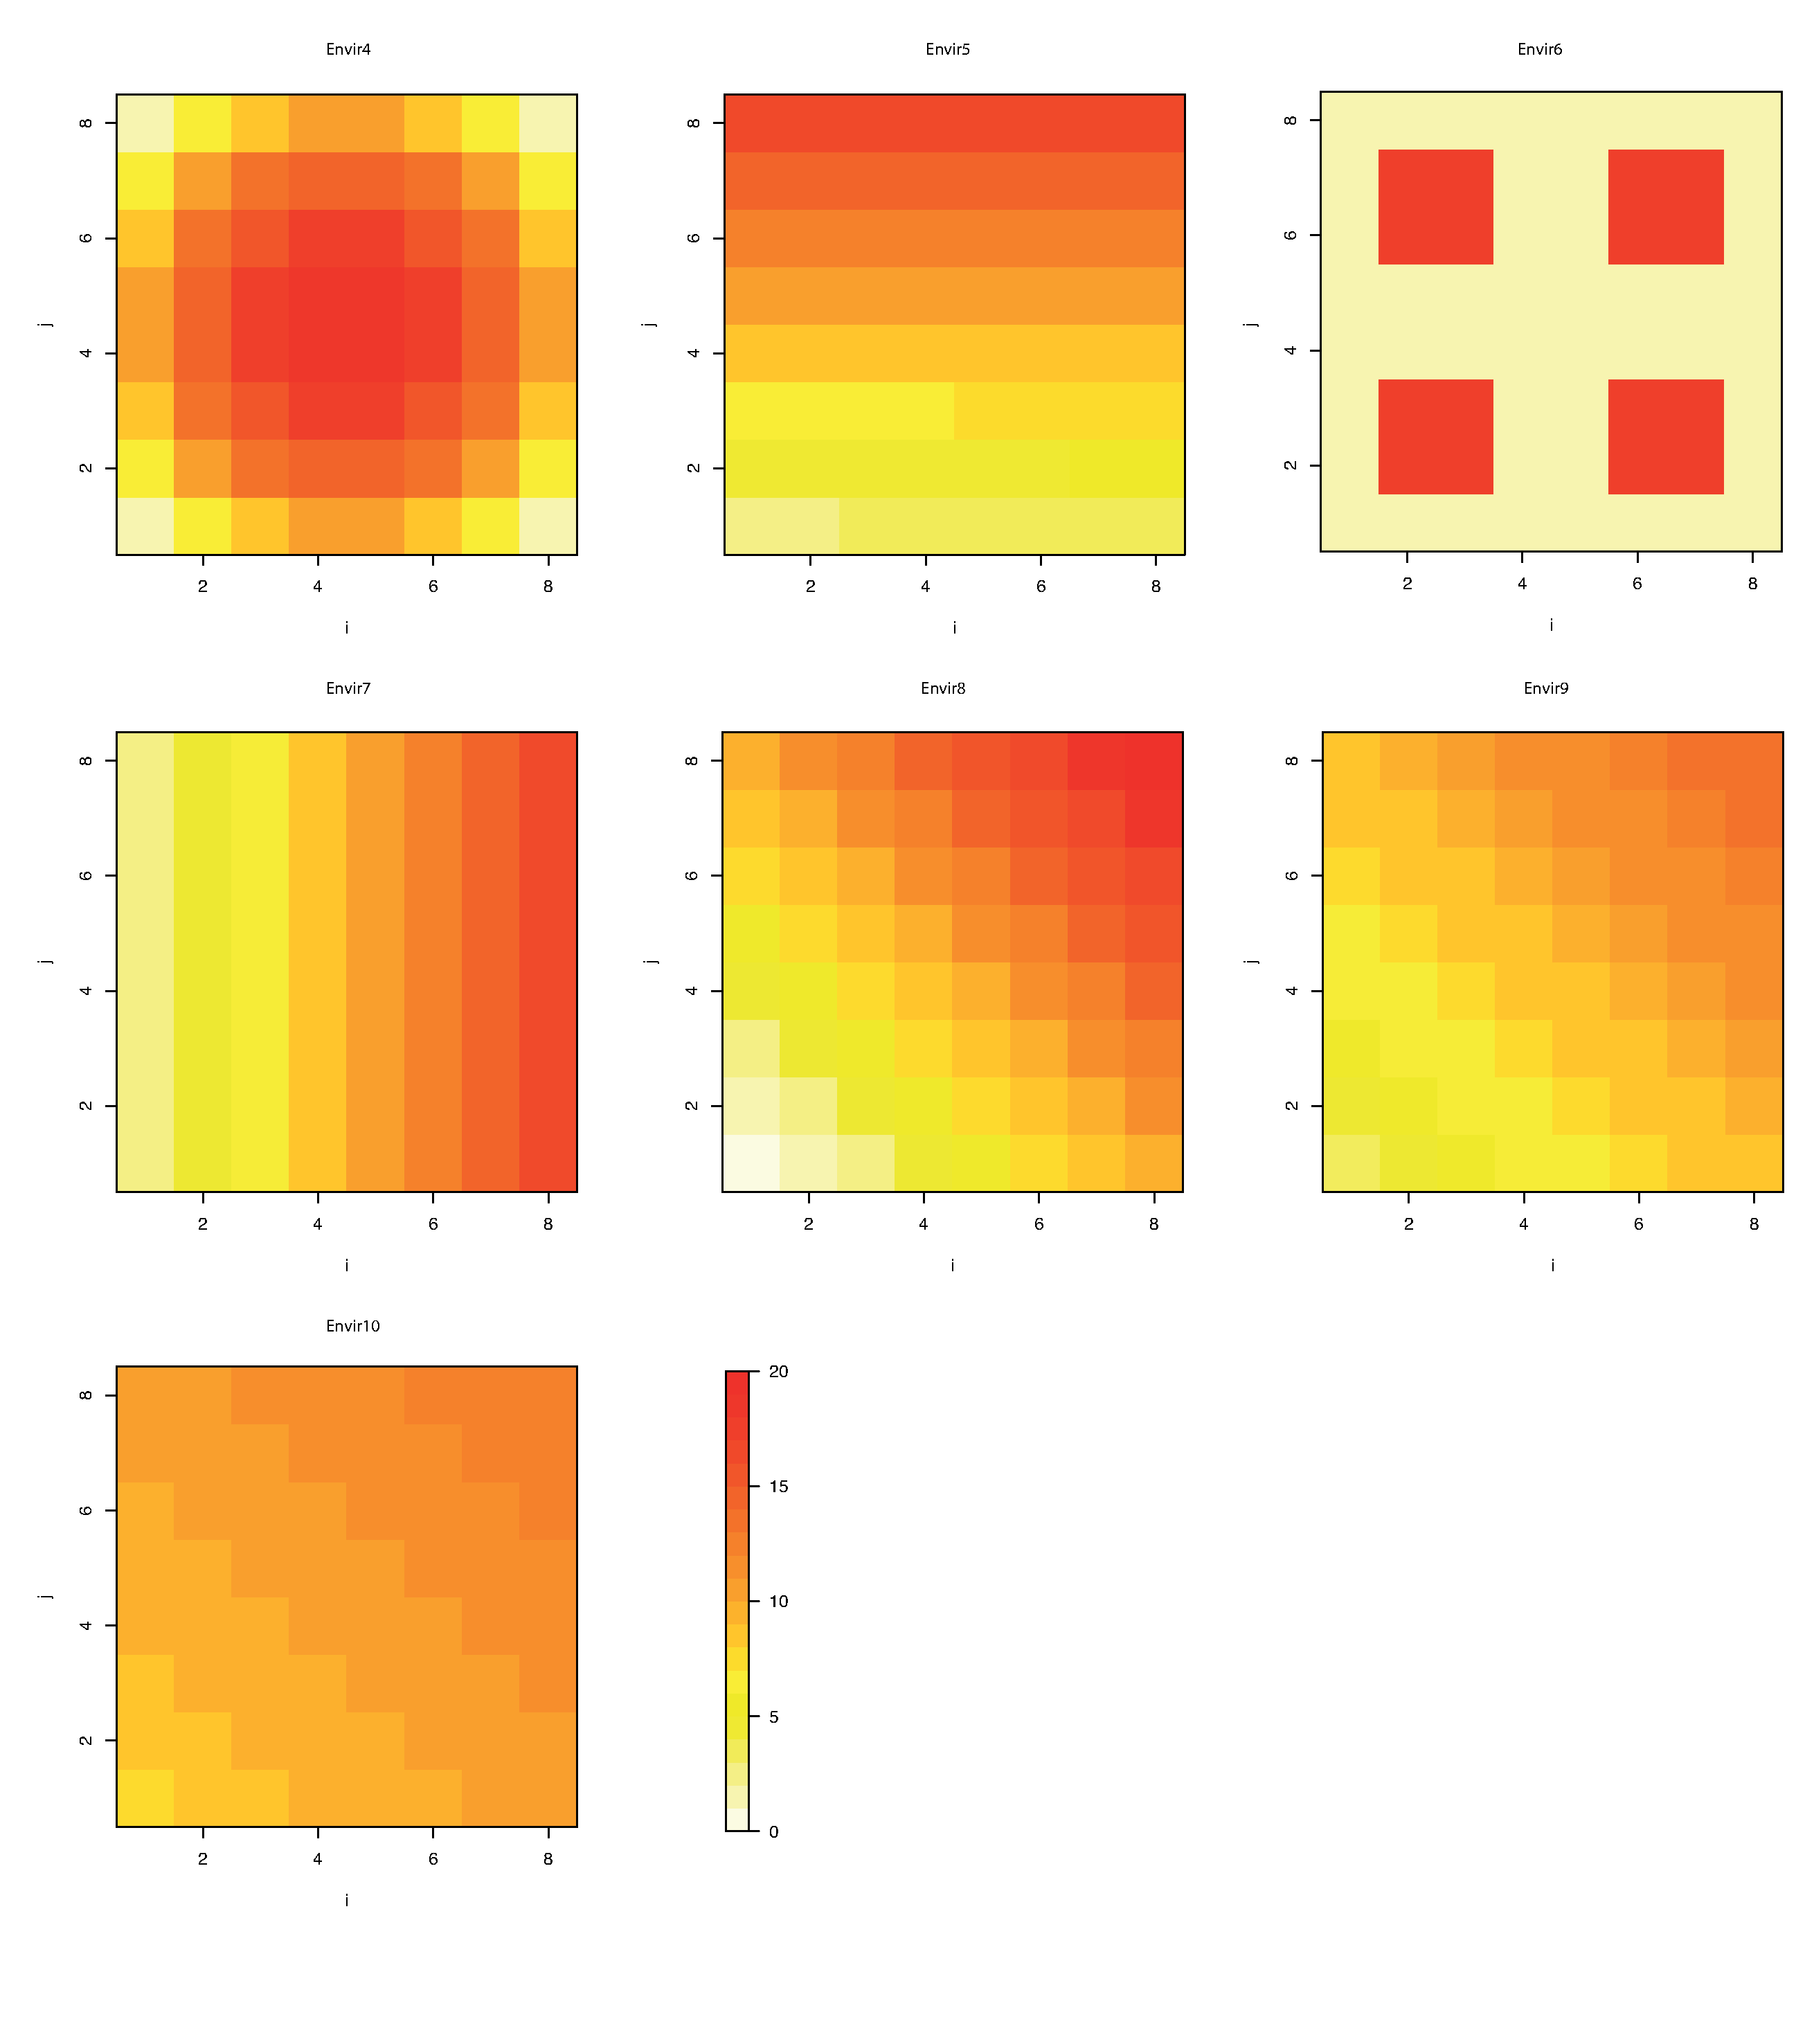
\includegraphics[height=0.8\textheight]{figures/environmentaldata.eps}
\end{center}
\caption{Graphical representation of mean environmental value for environment 4 to 10. Equation determining the environment is given in the main manuscript. Mean environmental value for environment 4, 5 and 6 are respectively equivalent to environment 1, 2 and 3.}%
\label{fig:simulatedenvir}%
\end{figure*}

\begin{figure*}[t]
\begin{center}
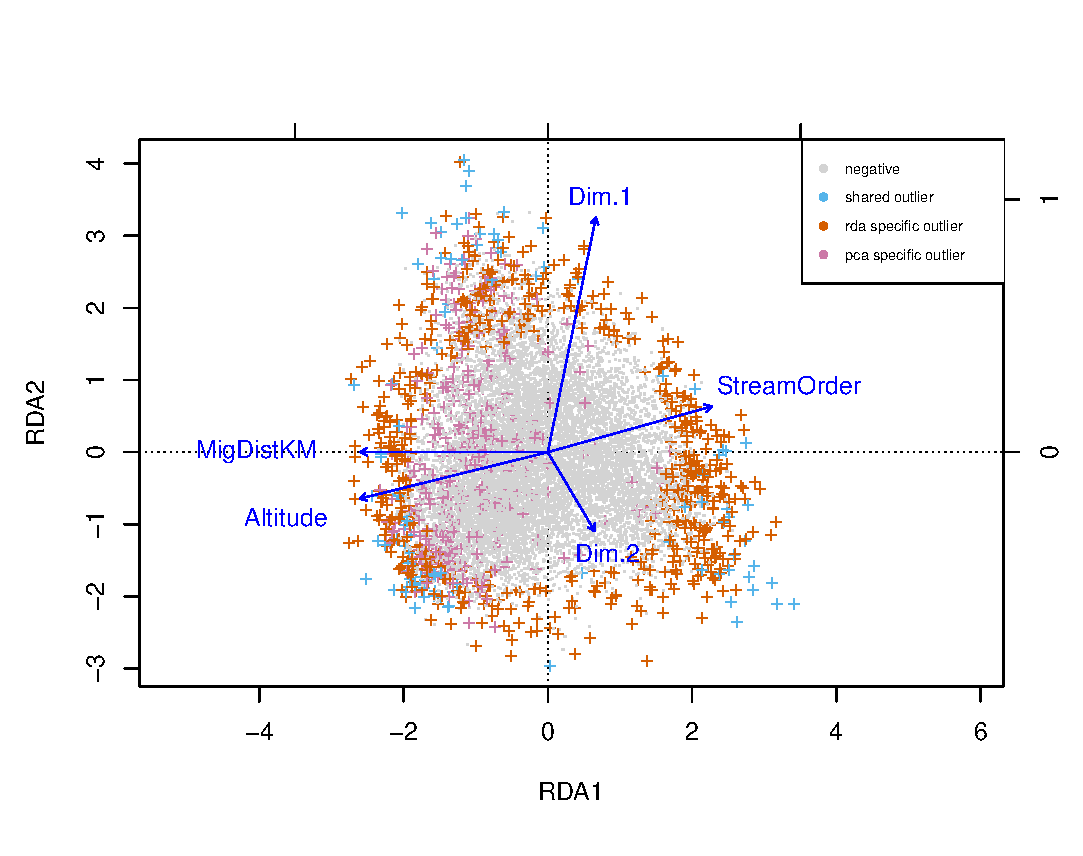
\includegraphics[height=0.6\textheight]{figures/salmon_rda.eps}
\end{center}
\caption{RDA genome scan on Chinook Salmon data. The first two axis RDA1 and RDA2 explain XX and XX\% of variance. Specific and shared outliers between PCA based method and RDA based method are differentially colored.}%
\label{fig:simulatedenvir}%
\end{figure*}


\end{document}
